\documentclass[../main.tex]{subfiles}
\usepackage{silence}
\usepackage{xr}
\NewDocumentCommand{\ExternalDocument}{m}{
	\externaldocument{#1}
	\typeout{No file chapters/#1.aux.}
}
\ExternalDocument{3-SOTA}
\ExternalDocument{2-Background}
\WarningFilter{glossaries}{No \printglossary or \printglossaries found}
\robExtConfigure{disable externalization}
\begin{document}
\ifSubfilesClassLoaded{%
	\graphicspath{{figures/7-Interpretability/}}%
	\setcounter{chapter}{6}%
	\mainmatter%
}{
	\graphicspath{{../figures/7-Interpretability/}}%
}
\chapter{Explaining with counterfactuals}\label{chap:counterfactuals}
\minitocpage
\section{Methods}
	We propose to use \glspl{gan} to generate counterfactuals points
	robustness
	\subsection{\glsfmtshortpl{gan} to generate counterfactuals}
		Counterfactual explanations aims to explain a prediction of a sample \(\symbf{x}\) by finding a minimal perturbation \(\delta\) in the data space that will change the prediction.
		The search of a counterfactual explanation can be formulated as an optimization problem (see \cref{eq:opt_cf})~\cite{wachter2017counterfactual}.
		A valid counterfactual is a counterfactual with added properties: \ref{item:cf_actionability}, \ref{item:cf_sparse}, and \ref{item:cf_data_manifold}.
		\Glspl{gan} are a deep learning architecture for generating new samples, it relies on two components a Generator \(G\) capturing the data distribution and a discriminator \(D\) estimating the realness of a sample~(see~\cref{sec:gan})~\cite{Goodfellow2014GAN}.
		As \glspl{gan} are good in capturing data distribution they can be used to generate counterfactuals respecting the \ref{item:cf_data_manifold} constraint.

		\begin{figure}[htbp]
			\centering
			\begin{tikzpicture}[inner sep=0pt, very thick]
				\node at (0,0) [square, draw, minimum size=1.5cm] (xin) {\(\symbf{x}\)};
				\node (gen) [right=1cm of xin.east, anchor=west, rounded rectangle, rounded rectangle west arc=none, draw, minimum height=1cm, minimum width=11mm] {\(G\)};
				\node (delta) [right=1.5cm of gen.east, anchor=west,square, draw, minimum size=1.5cm] {\(\delta\)};
				\node (add) [right=5mm of delta.east, anchor=west, draw, circle, minimum size=7.5mm] {};
				\draw (add.north) -- (add.south);
				\draw (add.west) -- (add.east);
				\node (xcf) [right=5mm of add.east, anchor=west,square, draw, minimum size=1.5cm] {\(x^{\text{CF}}\)};
				\node (cl1) [right=1cm of xcf.east, anchor=west, rounded rectangle, rounded rectangle west arc=none, draw, minimum height=1cm, minimum width=11mm] {\(\operatorname{Cl}\)};
				\node (cly) [right=6mm of cl1.east, anchor=west] {\(\hat{y}\)};
				\node (ycf) [right=1.5cm of cly.east, anchor=west] {\(y^{\text{CF}}\)};

				\node (dis) [below=7mm of cl1.south, anchor=north, rounded rectangle, rounded rectangle west arc=none, draw, minimum height=1cm, minimum width=11mm] {\(D\)};
				\node (realfake) at (dis.east -| cly.south)  {\(s\)};
				\node[align=left] (labelrealfake) at (realfake.east -| ycf.south) {0 \\ 1};

				\node (cl2) [above=7mm of cl1.north, anchor=south, rounded rectangle, rounded rectangle west arc=none, draw, minimum height=1cm, minimum width=11mm] {\(\operatorname{Cl}_{T}\)};
				\node (cl2y) at (cl2.east -| cly.north)  {\(\hat{y}_{T}\)};
				\node (ytissue) at (cl2y.east -| ycf.north) {\(y_{T}\)};

				\node (xreal) at (xcf.south |- dis.east) [draw, square, minimum size=1.5cm, double copy shadow={shadow xshift=-.5ex, shadow yshift=.5ex, opacity=.5}, fill=white] {\(\symcal{X}\)};

				\draw[-stealth] (xin.east) -- (gen.west);
				\draw[-stealth] (gen.east) -- node [midway, matrix, draw=none, anchor=center, yshift=0.6em] {
					\node[draw=none,minimum size=1.2em] {\(\symcal{M}\)}; \\
					\node[draw,fill=black,minimum size=1.2em] {};  \\
					\node[draw,fill=white,minimum size=1.2em] {};  \\
					\node[draw,fill=black,minimum size=1.2em] {};  \\
					\node[draw,fill=white,minimum size=1.2em] {};  \\
					\node[draw,fill=black,minimum size=1.2em] {};  \\
					\node[draw,fill=white,minimum size=1.2em] {};  \\
				} (delta.west);
				\draw[-stealth] (delta.east) -- (add.west);
				\draw[-stealth]  (xin.south) -- ++(0,-12mm) -| (add.south);
				\draw[-stealth] (add.east) -- (xcf.west);
				\draw[-stealth] (xcf.east) -- (cl1.west);
				\draw[-stealth] (xcf.east) -- ++(4mm, 0) |- ([yshift=2mm]dis.west);
				\draw[-stealth] ([yshift=-2mm]xreal.east) -- ([yshift=-2mm]dis.west);
				\draw[-stealth] (xcf.east) -- ++(4mm, 0) |- (cl2.west);
				\draw[-stealth] (cl1.east) -- (cly.west);
				\draw[-stealth] (cl2.east) -- (cl2y.west);
				\draw[-stealth] (dis.east) -- (realfake.west);
				\draw[stealth-stealth, dashed] (cly.east) -- node [midway,above, yshift=0.5ex] {\(\symcal{L}_{\operatorname{Cl}}\)}  (ycf.west);
				\draw[stealth-stealth, dashed] (cl2y.east) -- node [midway,above, yshift=0.5ex] {\(\symcal{L}_{\operatorname{Cl}_{T}}\)}  (ytissue.west);
				\draw[stealth-stealth, dashed] (realfake.east) -- node [midway,above, yshift=0.5ex] {\(\symcal{L}_{\text{GAN}}\)}  (labelrealfake.west);
			\end{tikzpicture}
			\caption[Architecture of the counterfactual \glsfmtshort{gan}]{Architecture of the counterfactual \glsfmtshort{gan}. The example \(x\), for which a counterfactual is searched, is passed through the generator \(G\) to obtain the optimal perturbation \(\delta\). This perturbation is added to the input to obtain the counterfactual point \(x^{\text{CF}}\). During the training phase, the counterfactual point is evaluated with two classifiers to ensure the point is classified to the desired class (\(\operatorname{Cl}\)) and belongs to the same tissue as the original point (\(\operatorname{Cl}_{T}\)). A critic \(D\) is used to ensure the generated point belongs to the original data distribution. }\label{fig:gan_cf}
		\end{figure}

		\Cref{fig:gan_cf} presents the overall architecture of the \gls{gan} used for generating counterfactual explanations.
		To obtain a counterfactual, the point \(\symbf{x}\) to explain is passed through the generator \(G\), a \gls{fcn} of \(l\) layers with \gls{relu} intermediate activation and no final activation, to obtain the perturbation \(\delta\).
		To ensure the \ref{item:cf_actionability} property a binary mask \(\symcal{M}\) is applied element-wise on the generated perturbation to specify which features can be changed.
		\begin{equation}
			\delta = G\left(\symbf{x}\right) \odot \symcal{M}
		\end{equation}
		The counterfactual point or explanation is obtained by adding this perturbation \(\delta\) to the original point: \(\symbf{x}^{\text{CF}} = \symbf{x} + \delta\).

		As \glspl{gan} are known for their training instabilities~\cite{Salimans2016ImprovedTF,Arjovsky2017TowardsPM}, we used a \gls{wgan} with gradient penalty (see~\cref{sec:gan})~\cite{WGANGP}.
		The WGAN-GP is trained by solving the following optimization problem:
		\begin{multline}
			\min_{G} \max_{D} \symcal{L}_{\text{WGAN}}\left(G,D\right) = \E_{x\sim p_{d}}\left[ D\left(x\right)\right] - \E_{x^{\text{CF}}\sim p_{g}}\left[ D\left(x^{\text{CF}}\right)\right] \\ + \lambda \E_{\tilde{x}\sim p_{g}}\left[ {\left( {\left\|\nabla_{\tilde{x}}D\left(\tilde{x}\right) \right\|}_{2} -1 \right)}^{2}\right] \label{eq:wgan_opt_cf}
		\end{multline}
		where \(p_{d}\) is the true data distribution, \(p_{g}\) is the distribution learned by the generator \(G\), \(\lambda\) is the penalty weight forcing the discriminator \(D\) to be a K-Lipschitz function, and \(\tilde{x}\) is a linearly interpolated point between \(x\) and \(x^{\text{CF}}\).
		The main desirata of a counterfactual is to change the predicted class of \(\symbf{x}\) from \(\hat{y}\) to \(y^{\text{CF}}\).
		The fullfilment of this constraint is achieved by adding a term \(\symcal{L}_{\operatorname{Cl}}\left(G,\operatorname{Cl}, y^{\text{CF}} \right) = \symcal{L}_{\text{CE}}\left(\operatorname{Cl}\left(x^{\text{CF}}\right),y^{\text{CF}}\right) \) to the optimization problem~(\cref{eq:wgan_opt_cf}), where \(\operatorname{Cl}\) is a pretrained classifier and \(\symcal{L}_{\text{CE}}\) the cross-entropy loss~(see~\cref{eq:ce_loss}).
		The \ref{item:cf_sparse} constraint of a counterfactual is obtained by adding a \(L_{1}\) regularization on the generated perturbation \(\delta\) to the optimization problem~(\cref{eq:wgan_opt_cf}): \(\symcal{L}_{\text{Reg}}\left(G\right) = \left\|G\left(x\right) \odot \symcal{M}\right\|_{1}\).
		More constraints can be added onto the generator by adding other loss terms to the optimization problem.
		For instance, in our scenario we added a loss term \(\symcal{L}_{\operatorname{Cl}_{T}}\left(G,\operatorname{Cl}_{T}, y_{T} \right) = \symcal{L}_{\text{CE}}\left(\operatorname{Cl}_{T}\left(x^{\text{CF}}\right),y_{T}\right)\) to ensure that the generated counterfactual belongs to the correct tissue type, where \(\operatorname{Cl}_{T}\) is a pretrained tissue classifier.
		Finally, the counterfactual \gls{wgan} is trained by solving the following optimization problem:
		\begin{multline}
			\min_{G} \max_{D} \symcal{L}_{\text{WGAN}}\left(G,D\right) + \symcal{L}_{\operatorname{Cl}}\left(G,\operatorname{Cl}, y^{\text{CF}}\right)\\ + \symcal{L}_{\operatorname{Cl}_{T}}\left(G,\operatorname{Cl}_{T}, y_{T}\right) + \symcal{L}_{\text{Reg}}\left(G\right)
		\end{multline}

	\subsection{Counterfactuals evaluation}
		distance, L0 to check the sparsity
		A realistic counterfactual should have points in its neighborhood that are classified the same.
		yNN proportion of point in the k nearest neighbors classified the same accuracy based on the kNN neighbors characterization \cite{Carla_CF}
		can also be visualized by projecting counterfactuals points onto the UMAP space obtained from the training data.
		Sucess rate / Accuracy are we able to change the label for all points
		UMAP evaluation + neighbors characterization

	\subsection{Getting a robust model: adversarial training}
		adversarial and counterfactuals close proximity (solve similar optimization problem).
		Prevent the GAN from finding adversarial --> make the classifier robust to adversarial examples
		achieved with adversarial training: opt problem
		algo

	\subsection{Adversarial Metrics}
		To evaluate model robustness, we used three metrics: model smoothness, margin decision~\cite{MarginDecision} and boundary thickness.
		The details of each metric is given below:
		\begin{description}[
				style=multiline,
				leftmargin=!,
				labelwidth=2.5cm
			]
			\item[Model smoothness]
				insensitiveness of the output to the input perturbation~\cite{MarginDecision}
				KL divergence
				smaller smoothness is better
			\item[Margin decision]
				This metric measure the distance of an example to the decision boundary~\cite{MarginDecision}.
				text version of the metric
				\begin{equation}
					g\left(\symbf{x}\right)_{y} - \max_{i \neq y} g\left(\symbf{x}\right)_{i}
				\end{equation}
				A higher margin decision is better.
			\item[Boundary thickness]
				Thick decision boundaries lead to improved performance
				thicker boundary helps improve robustness against adversarial examples
				\begin{equation}
					\left\|x - x^{\star}\right\|_{2} \int_{0}^{1} \symbb{1}\left\{ \alpha < g_{ij}\left(tx + \left(1-t\right)x^{\star} \right) < \beta\right\}
				\end{equation}
		\end{description}


\section{Preliminary results}
	\subsection{Adversarial study}
		what attacks we used PGD Linf cite package
		how did we choose epsilon (distance class)
		BN problems, consider models without batch normalization
		comparison of different models, justification problem BatchNorm
		present the different models
		identify the optimal number of training steps for each model
		compare different epsilon attacks
		targeted vs untargeted
		Metrics
		neighbors characterization
		\begin{figure}[htbp]
			\centering
			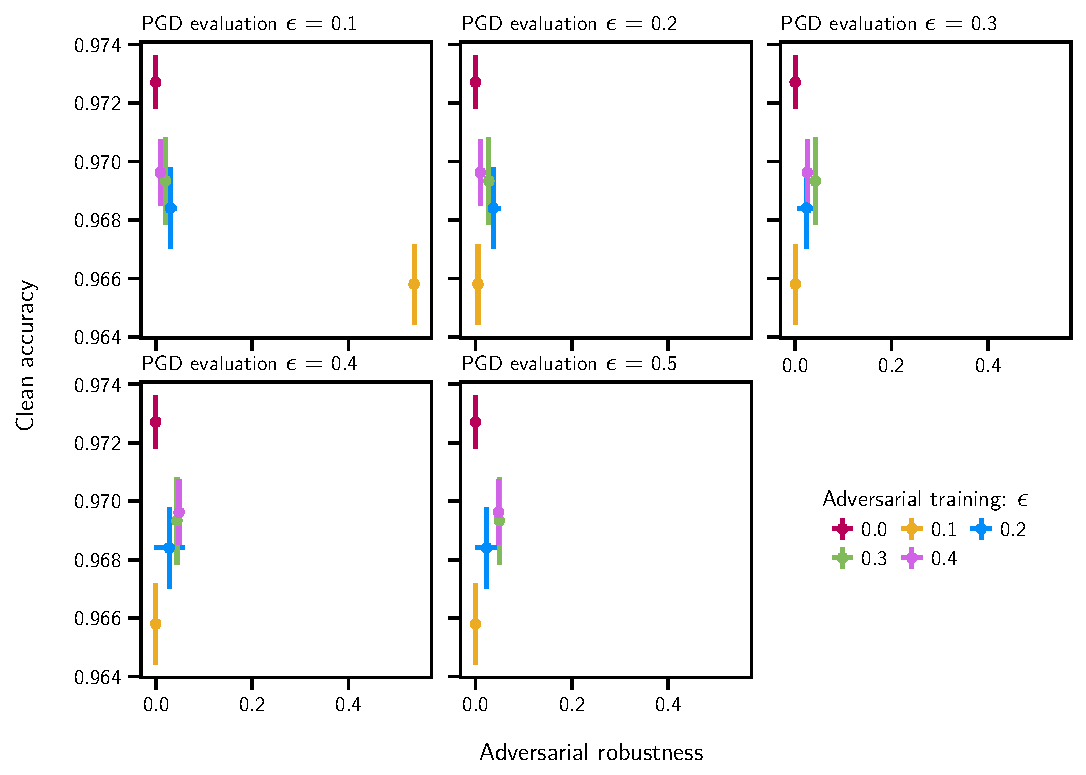
\includegraphics{MLP_BN_adversarial_tradeoff.pdf}
			\caption{MLP with BatchNorm adversarial tradeoff}\label{fig:mlp_bn_adv_tradeoff}
		\end{figure}

		\begin{figure}[htbp]
			\centering
			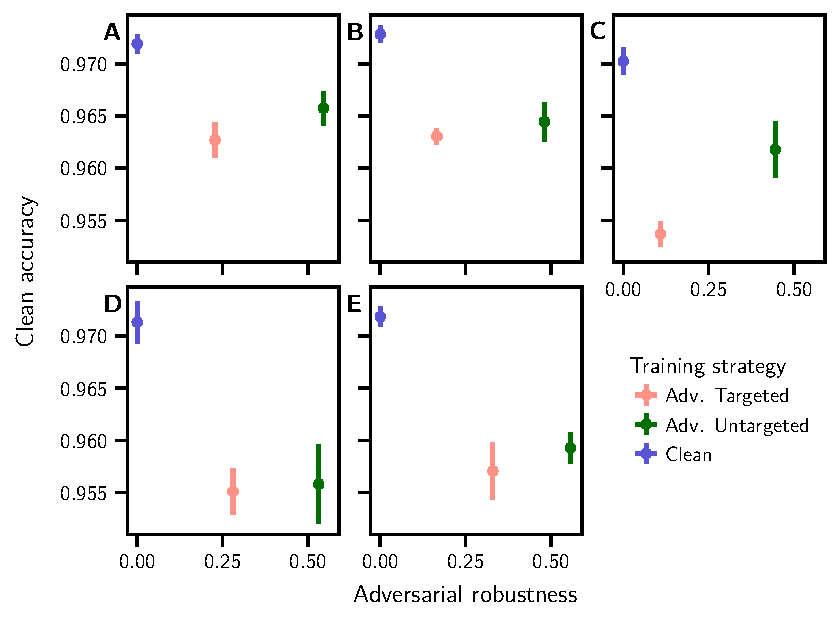
\includegraphics{adversarial_robustness_strategy.pdf}
			\caption{Adversarial robustness strategy}\label{fig:adv_robust_strat}
		\end{figure}

		\begin{landscape}
			\begin{figure}[htbp]
				\centering
				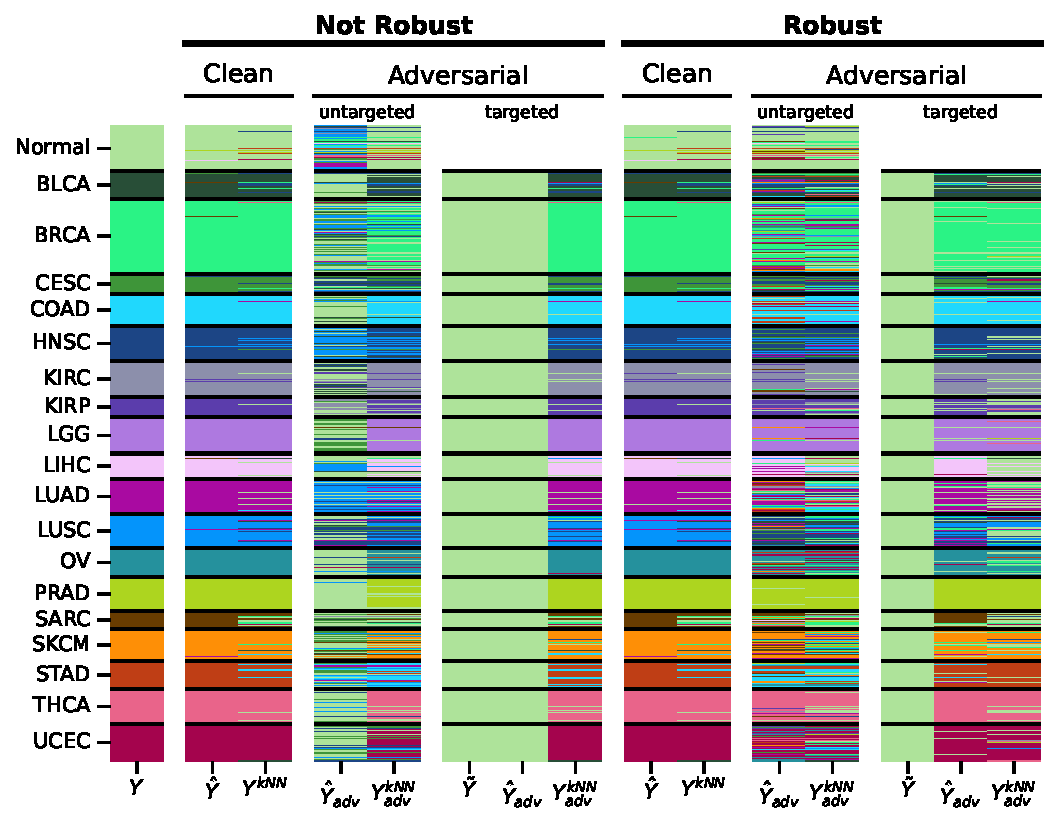
\includegraphics{MLP_BN_knn_comparison.pdf}
				\caption{MLP BatchNorm knn comparison}\label{fig:mlp_bn_knn_comp}
			\end{figure}
		\end{landscape}

		\cite{SzegedyZSBEGF13}
		\begin{table}[htbp]
			\sisetup{round-mode=places,round-precision=2}
			\caption[Adversarial metrics]{Some LEGEND, a robust model corresponds to a model that have been adversarially trained.}\label{tab:metrics_adv}
			\csvreader[
				no head,
				centered tabularray={%
						colspec={%
								Q[c,m]
								Q[si={table-format=2.2,table-number-alignment=center}, wd=1.4cm]%
								Q[si={table-format=2.2,table-number-alignment=center}, wd=1.4cm]%
								Q[si={table-format=2.2,table-number-alignment=center}, wd=1.4cm]%
								Q[si={table-format=2.2,table-number-alignment=center}, wd=1.4cm]%
								Q[si={table-format=2.2,table-number-alignment=center}, wd=1.6cm]%
								Q[si={table-format=2.2,table-number-alignment=center}, wd=1.6cm]%
							},%
						row{1-2} = {guard},
						row{2} = {c,m},
						row{3-Z} = {font=\small},
						row{1} = {font=\bfseries},
						cell{1}{2} = {r=1,c=2}{c, wd=2.8cm},
						cell{1}{4} = {r=1,c=2}{c, wd=2.8cm},
						cell{1}{6} = {r=1,c=2}{c, wd=3.2cm},
						hline{1} = {2-Z}{2pt},%
						hline{Z} = {2pt},%
						hline{2-3} = {1pt},%
						column{even} = {rightsep=2pt},
						column{odd[3-Z]} = {leftsep=2pt},
						cell{3-Z}{1} = {font=\normalsize}
					}
			]{%
				\ifSubfilesClassLoaded{%
					data/AdversarialMetrics.csv%
				}{%
					../data/AdversarialMetrics.csv%
				}%
			}{}{\csvlinetotablerow}
		\end{table}
	\subsection{Counterfactuals}








		counterfactuals, could we compare the proposed treatments with, when available, the treatment scheme of the patient.

\end{document}
